\documentclass[12pt,a4paper]{report}

\usepackage{float}
\usepackage{graphicx}
\usepackage{fancyhdr}
\usepackage{enumitem}
\usepackage{pgfplots}
\usepackage{datetime}
\usepackage{lastpage}
\usepackage[top=2cm,bottom=2cm,right=2cm,left=2cm]{geometry}

\pgfplotsset{compat=1.18}
\pagestyle{fancy}   
\lhead{Machines and Drives Report}
\rhead{Shawal Mbalire 21/U/0851}
\cfoot{Page~\thepage~of~\pageref{LastPage}}

\begin{document}

\begin{titlepage}
    \begin{center}
        \begin{figure}[H]
            \centering
            \includegraphics[width=0.5\textwidth]{muk.png}
        \end{figure}

        \vspace{20pt}

        \large COLLEGE OF ENGINEERING, DESIGN, ART AND TECHNOLOGY\\
        \vspace{10pt}
        DEPARTMENT OF ELECTRICAL AND COMPUTER ENGINEERING\\
        \vspace{10pt}
        BACHELOR OF SCIENCE IN ELECTRICAL ENGINEERING\\
        \vspace{10pt}
        SHAWAL MBALIRE\\
        \vspace{10pt}
        21/U/0851\\
        \vspace{20pt}

        \textbf{\Large MACHINES AND DRIVES I LAB REPORT}\\
        \vspace{20pt}

        % \begin{table}[H]
        %     \centering
        %     \begin{tabular}{|llc|}
        %         \hline
        %         \multicolumn{3}{|c|}{\textbf{Group Members}} \\ \hline
        %         \multicolumn{1}{|l|}{\textbf{S/N}} & \multicolumn{1}{l|}{\textbf{Name}} & \textbf{Registration Number} \\ \hline
        %         \multicolumn{1}{|l|}{1} & \multicolumn{1}{l|}{Amutuhire Judith} & 22/U/5773 \\ \hline
        %         \multicolumn{1}{|l|}{2} & \multicolumn{1}{l|}{Achola Loy Abor} & 22/U/5637 \\ \hline
        %         \multicolumn{1}{|l|}{3} & \multicolumn{1}{l|}{Agasha Moreen} & 22/U/5659 \\ \hline
        %         \multicolumn{1}{|l|}{4} & \multicolumn{1}{l|}{Aine Mugabe Hillary} & 22/U/5683 \\ \hline
        %         \multicolumn{1}{|l|}{5} & \multicolumn{1}{l|}{Ainembabazi Irene} & 22/U/21209/PSA \\ \hline
        %         \multicolumn{1}{|l|}{6} & \multicolumn{1}{l|}{Ajolo Precious Mercy} & 22/U/5696 \\ \hline
        %         \multicolumn{1}{|l|}{7} & \multicolumn{1}{l|}{Amara Alex} & 22/U/5752 \\ \hline
        %         \multicolumn{1}{|l|}{8} & \multicolumn{1}{l|}{Abraham Kizza} & 22/U/21313 \\ \hline
        %         \multicolumn{1}{|l|}{9} & \multicolumn{1}{l|}{Anena Cuthbert Wanitho} & 20/U/16043 \\ \hline
        %         \multicolumn{1}{|l|}{10} & \multicolumn{1}{l|}{Ankwasa Derrick} & 22/U/5780 \\ \hline
        %         \multicolumn{1}{|l|}{11} & \multicolumn{1}{l|}{Aransiola Oyindamola S O} & 21/X/20031/PS \\ \hline
        %         \multicolumn{1}{|l|}{12} & \multicolumn{1}{l|}{Arinaitwe Elastus} & 22/U/5798 \\ \hline
        %         \multicolumn{1}{|l|}{13} & \multicolumn{1}{l|}{Asiimwe Martha Serena} & 22/U/5814 \\ \hline
        %         \multicolumn{1}{|l|}{14} & \multicolumn{1}{l|}{Atuhura Joshua Wamani} & 22/U/5833 \\ \hline
        %         \multicolumn{1}{|l|}{15} & \multicolumn{1}{l|}{Bagoole Asadi} & 22/U/5858 \\ \hline
        %     \end{tabular}
        % \end{table}

       
        \vspace{20pt}

        \normalsize Instructor: Mr. Robinson Ntege\\
        \vspace{10pt}

        \normalsize \today
        \vspace{20pt}

    \end{center}
\end{titlepage}

\tableofcontents
\newpage

\listoffigures
\newpage

\listoftables
\newpage


\chapter{Experiment to determine the transformation ratio and the equivalent circuit parameters of a single phase transformer.}

\section{Objectives}
\begin{enumerate}[label=\roman*.]
    \item To determine the transformation ratio, k.
    \item To determine the equivalent circuit parameters.
\end{enumerate}

\section{List of Apparatus}
\begin{enumerate}[label=\roman*.]
    \item Single phase transformer
    \item Variac
    \item AC ammeters and voltmeters
    \item Wattmeter
\end{enumerate}

\section{Theory}
It is well known that the equivalent circuit of a single phase transformer can be approximately represented as shown below. The parameters $r_{0}$ and $x_{0}$ which take into account the two components of the no load current can be determined by conducting an open circuit test. The parameters $r_{1}$ and $x_{1}$ are determined from the short circuit test.
\begin{figure}[H]
    \centering
    \includegraphics[width=0.8\linewidth]{figure_1_1.jpeg}
    \caption{Single phase transformer equivalent circuit}
    \label{fig_1}
\end{figure}

\section{Procedures}
\subsection{Ratio Test}
\begin{enumerate}
    \item Connect the circuit shown in \ref{fig_2} below. 
    \begin{figure}[H]
        \centering
        \includegraphics[width=0.8\linewidth]{figure_2_2.jpeg}
        \caption{Single phase  transformer ratio test}
        \label{fig_2}
    \end{figure}
    \item Vary the output of the variac from 30V to 90V in steps of 90V.
    \item Measure and record the voltage on the low voltage and high voltage sides of the transformer.
    \item Record the results.
\end{enumerate}

\begin{table}[H]
    \centering
    \caption{Table of results for ratio test}
    \begin{tabular}{|l|l|l|}
    \hline
    LV Voltage , $V_{1}$ & HV Voltage, $V_{2}$ & $k=V_{2}/V_{1}$ \\ \hline
    30              & 60             & 2.00    \\ \hline
    40              & 80             & 2.00    \\ \hline
    50              & 100            & 2.00    \\ \hline
    60              & 130            & 2.17    \\ \hline
    70              & 150            & 2.14    \\ \hline
    80              & 170            & 2.13    \\ \hline
    90              & 185            & 2.06    \\ \hline
    \end{tabular}
    \end{table}

\subsection{Open Circuit Test}
\begin{enumerate}
    \item Make connections as shown in \ref{fig_3} below.
    \begin{figure}[H]
        \centering
        \includegraphics[width=0.8\linewidth]{figure_3_3.jpeg}
        \caption{Single phase transformer test}
        \label{fig_3}
    \end{figure}
    \item Apply rated voltage at the low voltage side of the transformer by varying the output of the variac.
    \item Measure and record the corresponding power input, W, on the LV side, the power factor and the voltage on the HV side.
    \item The procedure is repeated for different input voltages.
    \item The results are recorded in the table below.


\begin{table}[H]
    \centering
    \caption{Table of results for open circuit test}
    \begin{tabular}{|l|l|l|l|l|}
    \hline
    $V_{1}$ & $P_{0}$  & $I_{0}$  & $V_{2}$  & $cos\Phi_{0}=P_{0}/(V_{1}I_{0})$ \\ \hline
    30 & 10  & 1.5 & 48  & 0.2222          \\ \hline
    40 & 50  & 4.3 & 150 & 0.2907          \\ \hline
    50 & 210 & 18  & 162 & 0.2333          \\ \hline
    55 & 360 & 37  & 180 & 0.1769          \\ \hline
    \end{tabular}
    \end{table}
    \item Determine the open circuit parameters of your circuit\\
    \\
    \textbf{\textit{The open circuit parameters are tabulated in the table above}}
\end{enumerate}
\subsection{Short Circuit Test}
\begin{enumerate}
    \item Make the connections as shown in the \ref{fig_4} , with the LV side of the transformer short-circuited.
    \begin{figure}[H]
        \centering
        \includegraphics[width=0.8\linewidth]{figure_4_4.jpeg}
        \caption{Short circuit single phase transformer tests}
        \label{fig_4}
    \end{figure}
    \item Apply an input voltage, $V_{1}$ so that the rated current flows on the LV side of the transformer.
    \item Measure and record the power input, $P_{SC}$, the power factor, and the corresponding current, $I$ on the HV.
    \item Ensuring the input voltage does not exceed 8\% of the rated HV voltage.
    \item THe procedure is repeated for different lower values of short circuit currents, $I_{SC}$.
    \item The results are tabulated below.


\begin{table}[H]
\centering
    \caption{Table of results for short circuit tests}
    \begin{tabular}{|l|l|l|l|l|}
    \hline
    $V_{1}$ & $I_{SC}$  & $P_{SC}$ & $I$    & $cos\Phi=P_{SC}/(V_{1}I)$ \\ \hline
    2  & 0    & 0   & 0    & 0.0000         \\ \hline
    4  & 2    & 0   & 1    & 0.0000         \\ \hline
    6  & 8    & 5   & 4    & 0.2083         \\ \hline
    8  & 11   & 15  & 5.2  & 0.3606         \\ \hline
    10 & 14   & 25  & 7.5  & 0.3333         \\ \hline
    12 & 17   & 40  & 9    & 0.3704         \\ \hline
    14 & 20   & 60  & 10   & 0.4286         \\ \hline
    16 & 24   & 80  & 12   & 0.4167         \\ \hline
    18 & 26.5 & 110 & 13.5 & 0.4527         \\ \hline
    20 & 30   & 130 & 15   & 0.4333         \\ \hline
    \end{tabular}
    \end{table}
    \item Comment on your results. Determine the short circuit parameters of the transformer.\\
    \\
    \textbf{\textit{For small variation in voltages, there's a significant increase in the current. The short circuit parameters are tabulated in the table above}}
\end{enumerate}  
\chapter{Experiment to determine parameters and performance characteristics of Induction Motors.}
\section{Objectives}
\begin{enumerate}
    \item To determine equivalent circuit parameters of the induction motor from measurements.
    \item To predict the performance characteristics of the motor.
\end{enumerate}

\section{List of Apparatus}
\begin{enumerate}
    \item Power supply mod AV -1/V
    \item 4 Variable resistors RC3-PT
    \item Multifunctional digital instrument AZ VIP 10/EV 
    \item Digital Torque and speed measurement unit Um-G1/EV 
    \item 3 phase induction motor mod P-4/EV
\end{enumerate}

\section{Theory}
Induction motors operate by using a rotating magnetic field from the stator to induce currents in the rotor, generating torque. Key motor parameters—like stator and rotor resistances, reactances, and magnetizing reactance—are identified through standard tests: the no-load test, blocked rotor test, and load test. The no-load test evaluates magnetizing current and rotational losses, while the blocked rotor test (with the rotor prevented from rotating) is used to determine rotor and stator resistance and leakage reactances. The load test then assesses the motor’s efficiency, power factor, and torque-speed performance under actual load conditions.\\
\\
From these tests, an equivalent circuit model can be constructed, offering insights into the motor’s efficiency, slip, and torque characteristics. This model helps engineers predict motor behavior, optimize performance, and select the right motor for specific applications.

\section{Procedure}
\subsection{Light Running Test}
\begin{enumerate}
    \item Connect the machine as shown in the fig below.
    \begin{figure}[H]
        \centering
        \includegraphics[width=0.8\linewidth]{figure_5_5.jpeg}
        \caption{Light running test: without load}
        \label{fig_5}
    \end{figure}
    \item Start the motor by applying normal frequency, reduced voltage and gradually increase the input voltage to its rated value.
    \item Note down the readings for voltage, current, power and speed at different voltages.
    \item The results are tabulated.


\begin{table}[H]
\centering
    \caption{Table of results for light running test}
    \begin{tabular}{|l|l|l|l|l|l|l|}
    \hline
    $V_{1}(V)$ & $I(A)$  & $W_{1}(W)$ & $W_{2}(W)$ & $W_{3}(W)$ & $n(rpm)$ & $\rho=(W_{1}-W_{2})/W_{1}$ \\ \hline
    30    & 0.584 & 3.80  & 4.40  & 3.80  & 0      & -0.1579      \\ \hline
    40    & 0.911 & 9.70  & 10.40 & 9.20  & 0      & -0.0722      \\ \hline
    50    & 1.246 & 18.30 & 19.40 & 17.30 & 0      & -0.0601      \\ \hline
    60    & 1.597 & 31.00 & 30.20 & 27.90 & 89     & 0.0258       \\ \hline
    70    & 1.890 & 45.00 & 44.00 & 40.60 & 320    & 0.0222       \\ \hline
    80    & 0.870 & 33.30 & 33.50 & 29.70 & 2601   & -0.0060      \\ \hline
    90    & 0.673 & 27.50 & 29.20 & 24.80 & 2779   & -0.0618      \\ \hline
    100   & 0.566 & 26.50 & 28.30 & 24.20 & 2839   & -0.0679      \\ \hline
    110   & 0.523 & 27.20 & 27.10 & 23.00 & 2869   & 0.0037       \\ \hline
    \end{tabular}
    \end{table}
    \item Plot V against n.
\end{enumerate}

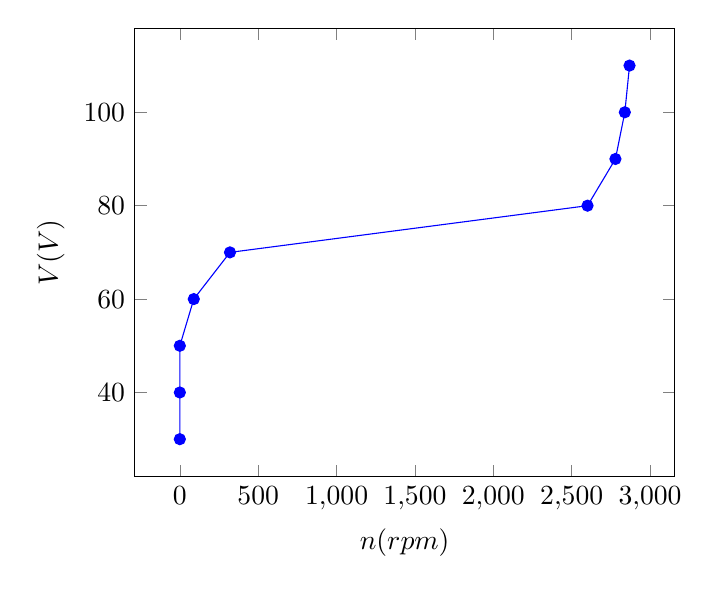
\begin{tikzpicture}
    \begin{axis}[
        compat=1.18,
        xlabel = $n(rpm)$,
        ylabel = $V(V)$,
    ]
    \addplot [
        table/row sep=\\,
        mark=*,
        color=blue,
    ]
    table {
        n     V  \\
        0     30 \\
        0     40 \\
        0     50 \\
        89    60 \\
        320   70 \\
        2601  80 \\
        2779  90 \\
        2839  100 \\
        2869  110 \\
    };
    \end{axis}
\end{tikzpicture}

\subsection{Blocked Rotor}
\begin{enumerate}
    \item The connection is setup as shown below, block the rotor with a load cell.
    \begin{figure}[H]
        \centering
        \includegraphics[width=0.8\linewidth]{figure_6_6.jpeg}
        \caption{Blocked rotor}
        \label{fig_6}
    \end{figure}
    \item Measure:
    \begin{enumerate}[label=\roman*.]
        \item the torque\\
        \\
        torque = 0.26 Nm
        \item the force\\
        \\
        force = 0.96 kg
        \item Mechanical Power Developed 
         P(W) = T(Nm) $\omega$\\
         \\
         where $\omega = \frac{2 \pi n}{60}$\\
         \\
         using the least value of n at V = 50V\\
         \\
         n = 80 rpm\\
         \\
         $$\omega = \frac{2 . \pi . 80 }{60}$$
         $$\omega = 8.3776$$
         $$P = 0.26 . 8.3776$$
         $$P = 2.178W$$
         
    \end{enumerate}
\end{enumerate}
\chapter{Errors}

In conducting practical tests on transformers and induction motors, various sources of errors can affect the accuracy of measurements and results. Key sources of errors in transformer and motor testing include:

\section{Sources of Errors}

\begin{enumerate}
    \item \textbf{Instrument Accuracy}: Inaccuracies in voltmeters, ammeters, and wattmeters can lead to measurement errors during open and short circuit tests.
    \item \textbf{Connection Errors}: Poor connections or loose terminals can cause significant deviations in test results, especially during the high-current blocked rotor test.
    \item \textbf{Temperature Effects}: Changes in winding resistance due to temperature variations can affect results in short circuit and blocked rotor tests.
\end{enumerate}

\section{Error Minimization}

To minimize errors during the experiments, the following steps should be taken:

\begin{enumerate}
    \item \textbf{Instrument Calibration}: Ensure all measuring instruments are calibrated before testing to reduce reading errors.
    \item \textbf{Secure Connections}: Tighten all connections securely to avoid contact resistance that could affect results.
    \item \textbf{Temperature Control}: Conduct tests at stable temperatures or record temperature data to account for changes in resistance.
\end{enumerate}

\chapter{Conclusion}

The practical lab sessions on transformer and induction motor testing provided a solid foundation for understanding core principles of machine characteristics. By performing open and short circuit tests on transformers, we were able to accurately determine parameters like the equivalent impedance and transformer ratio. The light running and blocked rotor tests on induction motors allowed us to determine their key characteristics, such as slip and torque, under different operating conditions.

Overall, the experiments highlighted the importance of accurate measurement techniques, error minimization, and methodical setup for obtaining reliable data on machine performance. These hands-on exercises are crucial for developing practical skills in electrical machine testing and diagnostics.

\nocite{*}            
\bibliographystyle{ieeetr}  
\bibliography{ref} 


\end{document}